% ========== Config ========== %

\documentclass{article}

\usepackage{fancyhdr} % draw header and footer separations
\usepackage{lastpage} % get last page number
\usepackage[super]{natbib} % format references
\usepackage{url} % pretty wrap url
\usepackage{indentfirst} % indent every paragraph
\usepackage{hyperref} % color url
\hypersetup{urlcolor=blue, colorlinks=true}
\usepackage{pythonhighlight} % python syntax highlighting
\usepackage{amsmath} % equations
\usepackage{ amssymb } % symbols
\usepackage{graphicx} % images
\usepackage[left=2cm, right=2cm, bottom=3cm, top=3cm]{geometry} % margin settings
\usepackage{alltt}
\renewcommand{\ttdefault}{txtt}


\pagestyle{fancy}
\fancyhead[L]{DAT 510 - Security and Vulnerability in Networks}
\fancyhead[R]{Assignment 2}
\fancyfoot[C]{ \thepage / \pageref{LastPage} }
\fancyfoot[L]{ T\'eo Bouvard }

\renewcommand{\headrulewidth}{0.4pt}
\renewcommand{\footrulewidth}{0.4pt}


% ========== Meta ========== %

\title{\textbf{Secure Communication Protocols}}
\author{}
\date{}


% ========== Document ========== %

\begin{document}

\maketitle \thispagestyle{fancy}

\begin{abstract}
    In this assignment, we implement a secure communication protocol consisting of three consecutive steps. First, we use Diffie-Hellman\cite{Diffie76newdirections}\cite{Graham78securecommunications} key exchange to craft a shared private key between two actors using public key cryptography. We then use an implementation of the Blum Blum Shub\cite{Blum1986} algorithm to generate a cryptographically strong pseudo-random shared private key, using the previously exchanged key as seed. Finally, we use the generated random key to encrypt and decrypt messages between the two actors using AES\cite{Daemen99aesproposal} ciphers.
\end{abstract}

\section{Introduction}

Our main goal is to be able to communicate secret data over an unsecure communication channel. To do so, we have to encrypt our data before sending it, and decrypt it after recieving it, so that it only appears encrypted on the communication channel.
To perform these encryptions, we want to use a symmetric cipher allowing us to efficiently compute ciphertext from plaintext and vice versa. Before using symmetric encryption, we have to solve the key exchange problem, because we still need to communicate the private key between the two actors over an unsecure channel.
One answer to this first problem is to use public-key cryptography, and more specifically the Diffie-Hellman key exchange protocol. 

\subsection{Diffie-Hellman}

This key exchange scheme allows us to create a shared private key by only communicating public data. It relies on the computational difficulty of computing discrete logarithms. It has been formulated in 1976 by Whitfield Diffie and Martin Hellman\cite{Diffie76newdirections}\cite{Graham78securecommunications}. We use it to generate a first shared private key between two actors, Alice and Bob.

\subsection{Blum Blum Shub}

To increase the strength of the exchanged key, we use it as a seed to a cryptographically strong pseudo-random number generator. The chosen stream generator is Blum Blum Shub\cite{Blum1986}, which outputs the least significant bit of $x_{{n+1}}$ at each step of the following sequence.

\begin{equation*}
    x_{n+1}=x_{n}^{2} \bmod M
    \quad \quad \text{with $x_{0} = \text{seed}$, $M$ the product of two large primes $p$ and $q$}
\end{equation*}

\subsection{Advanced Encryption Standard}

To encrypt their messages, Alice and Bob can now use a symmetric cipher with their shared private key. Here, we use AES in Electronic Code Book mode. Now that Alice and Bob exchanged their keys, they could use any symmetric cipher and mode of operation. 

Using these cryptographic primitves, we implement a secure communication protocol allowing Alice and Bob to communicate data privately.

\section{Design and Implementation}

\subsection{Diffie-Hellman}

The python implementation of the Diffie-Hellman key exchange is fairly straightforward. There are two main steps in this scheme : creating a public key from our private key, and combining the other party's public key with our private key to generate the shared private key. These two steps are represented by the two main modes of operation of \verb+keygen.py+ : generate and merge, to be passed to the \verb+--mode+ argument. When running the script in \verb+--mode generate+, the main function used is the following.

\bigskip
\begin{python}
def pubkeygen(prime, root, secret):
    assert(is_prime(prime))
    assert(is_primitive_root(root, prime))

    return pow(root, secret, prime)
\end{python}
\bigskip

And when used in \verb+--mode merge+, the main computation is done in this function.

\bigskip
\begin{python}
def shared_secret_key(secret, other_public_key, prime):
    return pow(other_public_key, secret, prime)
\end{python}
\bigskip

Note that in both functions, we use the \verb+pow()+ method with three arguments rather than exponentiating and then taking the modulo. This is because on large numbers, the \verb+pow()+ method is significantly faster at computing the modulo than the raw computation of exponentiation followed by division. This is demonstrated in Figure \ref{fig:pow_speed}. 
This program is designed to accept decimal or hexadecimal representation of integers for the \verb+-{}-secret+, \verb+--prime+, \verb+--root+, and \verb+--public+ arguments.

The rest of the script is mostly dedicated to argument parsing, parameters loading and tests. The tests are run when using the script in \verb+--mode test+. The test data comes from the RFC 5114\cite{rfc5114} memo which describes standard Diffie-Hellman groups and their associated test data. Results of the tests can be found in Table \ref{tab:diffie}. The default group used by the script if no \verb+--prime+ and \verb+--root+ are passed is the 2048-bit MODP Group with 256-bit Prime Order Subgroup which can be found in the memo. 

Further specification for the other command line arguments can be found in the \verb+README.pdf+ file.

\subsection{Blum Blum Shub}

The main computation of the BBS algorithm is also quite simple, as bits are generated incrementally by taking the least significant bit of each modular exponentiation. The generated bits are then merged together and interpreted as a binary number.

\bigskip
\begin{python}
def generate_random(seed, size):

    bits = []

    for _ in range(size):
        seed = pow(seed, 2, M)
        bits.append(bin(seed)[-1])
    
    return int(''.join(bits), 2)
\end{python}
\bigskip

Although testing for statisical randomness usually involves a series of tests \cite{rukhin2001statistical}, we can visually check for pseudo-randomness by looking at the bitmap created by the generated bits. If we do not identify any regular pattern, we can assume that the randomness is reasonable for the key to be secure enough. This bitmap test can be seen in Figure \ref{fig:bitmap_bbs}.

\subsection{Advanced Encryption Standard}

The implementation of a symmetric cipher is not part of this assignment as it has already been done in Assignment 1. We choose AES for its ingenuity and subsequent popularity, and we use the Electronic Code Book mode of operation so that we do not have to transfer initialization vectors or nonces with the message. In a real-world application, we would prefer to use another mode as ECB is semantically insecure. Given a plaintext, ECB will always produce the same ciphertext each time. For a small amount of short text messages, this mode of operation is secure enough for our protocol.
  
\bigskip
\begin{python}
def encrypt(plaintext, key):
    cipher = AES.new(key, AES.MODE_ECB)
    if len(plaintext) % 16 != 0:
        plaintext = pad(plaintext, 16)
    ciphertext = cipher.encrypt(plaintext)
    return ciphertext
\end{python}
\bigskip

For encryption, we have to pad the plaintext if it does not fit the block size (16 bytes, 128 bits) as AES is a block cipher. During the decryption process, we unpad the decrypted ciphertext in the similar way. 

\bigskip
\begin{python}
def decrypt(ciphertext, key):
    cipher = AES.new(key, AES.MODE_ECB)
    plaintext = cipher.decrypt(ciphertext)
    if len(plaintext) % 16 != 0:
        plaintext = unpad(plaintext, 16)
    return plaintext
\end{python}
\bigskip

Although most of the work here is done by an external library \cite{pycryptodome}, we can still test the global implementation by using NIST test data \cite{nist:test}. This is done in Table \ref{tab:aes}.

\subsection{Putting it all together}

Now that we have seen how the different primitives are implemented, we can combine them to create the secure communication protocol we were seeking. To demonstrate how this can be done, a shell script describing a usecase is given. The file \verb+demo.sh+ serves as an example of how these primitives can be used in a modular way. Users may chose to run the programs quietly, or in verbose mode to display the parameters used. They may chose to redirect output to files. They may chose to change the parameters of the different primitives. This demo shell script is POSIX-compliant and should run on any reasonable shell. 
  
The other shell script provided, \verb+test.sh+, allows to run the implementation tests of the different primitives. 

\section{Test Results}

Table \ref{tab:diffie} shows the equivalence of test data from RFC 5114 \cite{rfc5114} and keys generated by our own implementation. The test data can be found in the \verb+files/2048-bit MODP Group+ folder.


Figure \ref{fig:pow_speed} shows the speed comparison of modular exponentiation methods. We observe exponential time complexity as the exponent gets larger using naive computation, whereas \verb+pow()+ remains nearly constant time.

\begin{figure}[h]
    \centering
    \begin{minipage}[t]{0.45\textwidth}
        \centering
        
\includegraphics[width=0.8\textwidth]{img/bitmap_bbs.png}
        \caption{Bitmap representation of a generated pseudo-random number}
        \label{fig:bitmap_bbs}
    \end{minipage}\hfill
    \begin{minipage}[t]{0.45\textwidth}
        \centering
        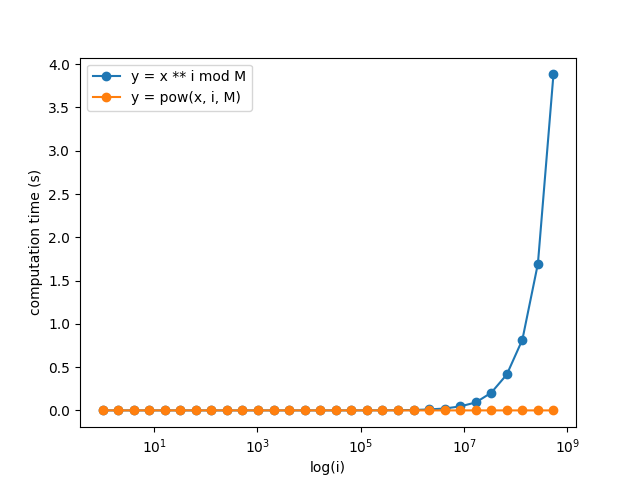
\includegraphics[width=\textwidth]{img/pow_speed.png}
        \caption{Modular exponentiation speed comparison}
        \label{fig:pow_speed}
    \end{minipage}
\end{figure}

\begin{table}[h]
    \begin{center}
        \begin{tabular}{|c| c c|} 
            \hline
            \textbf{Initiator} & \textbf{Public key equivalence} & \textbf{Shared private key equivalence} \\
            \hline
            A & \checkmark & \checkmark \\
            B & \checkmark & \checkmark \\
            \hline
        \end{tabular}
    \end{center}
    \caption{Comparing IETF test data to our implementation} \label{tab:diffie}
\end{table}

Table \ref{tab:aes} shows the equivalence between NIST test data \cite{nist:test} and data generated with our implementation using pycryptodome's AES cipher. The keys, ciphertexts and plaintexts used can be found in the \verb+files/AES_test_data+ folder.

\begin{table}[h]
    \begin{center}
        \begin{tabular}{|c c c|} 
            \hline
            \textbf{Key Length} & \textbf{Plaintext equivalence} & \textbf{Ciphertext equivalence} \\
            \hline
            128 bits & \checkmark & \checkmark \\
            192 bits & \checkmark & \checkmark \\
            256 bits & \checkmark & \checkmark \\
            \hline
        \end{tabular}
    \end{center}
    \caption{Comparing NIST test data to our implementation} \label{tab:aes}
\end{table}


\begin{figure}[h]
    \centering
    \begin{minipage}[t]{0.45\textwidth}
        \centering
        \frame{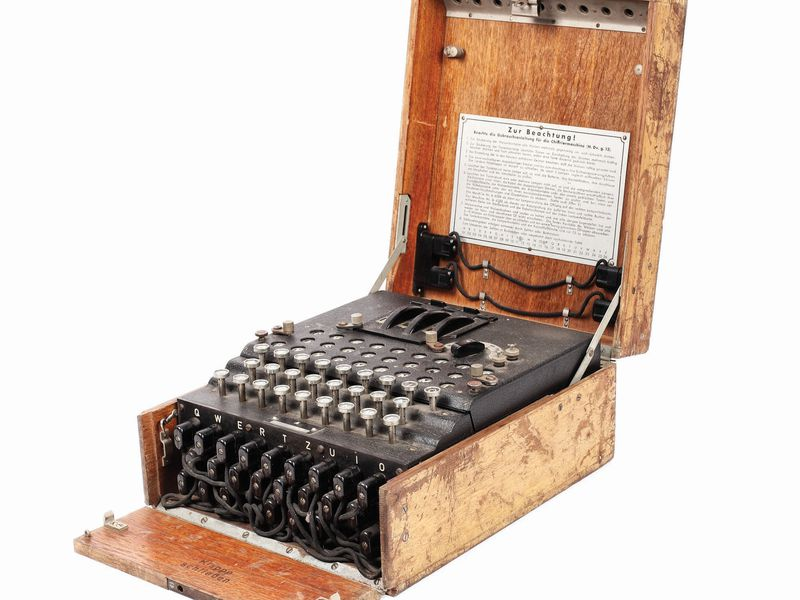
\includegraphics[width=\textwidth]{img/enigma.jpg}}
        \caption{Original image}
        \label{fig:original_image}
    \end{minipage}\hfill
    \begin{minipage}[t]{0.45\textwidth}
        \centering
        \frame{
\includegraphics[width=\textwidth]{img/encrypted_enigma.jpg}}
        \caption{Encrypted image using AES-ECB}
        \label{fig:encrypted_image}
    \end{minipage}
\end{figure}

\section{Discussion}

The key generation using Diffie-Hellman with a 2048-bit group is pretty much unbreakable with the current technology as it is estimated that an academic team can break a 768-bit prime and that a nation-state can break a 1024-bit prime \cite{weakdh15}. This is arguably the most secure part of our protocol. 

With a 2048-bit group, the exponent could be as large as $(2^{2048}-1) \sim 10^{616}$, which would take roughly $10^{170}$ years to compute with naive exponentiation. The \verb+pow()+ method is not only convenient, it is required for the program to complete.


Blum blum shub is slow and not practically secure (https://crypto.stackexchange.com/questions/3454/blum-blum-shub-vs-aes-ctr-or-other-csprngs)

ECB not secure
https://blog.filippo.io/the-ecb-penguin/

\section{Conclusion}


% ========== References ========== %

\bibliographystyle{unsrtnat}
\bibliography{sources}

\end{document}



